%notfulltexdoc
\section{Theory}
\subsection{The Accelerometer}
The STM32F407 Discovery board is equipped with an accelerometer which measures acceleration on three
axes. The accelerometer is a peripheral that communicates with the Discovery's CPU via the Serial
Peripheral Interface (SPI), where the Discovery is configured as Master and the accelerometer
peripheral is configured as Slave. Since the Discovery does not transmit anything to the
accelerometer, only its SPI RX line is in use, whereas only the SPI TX line is used on the
accelerometer. The Discovery and the accelerometer share a clock, generated by the Discovery's CPU
(because it is configured as the Master device), and share a common ground.\\\\
The directions over which accelerations are measured by the device are shown in
\hyperref[fig:accelaxes]{Figure \ref{fig:accelaxes}}.\\\\
\begin{figure}[h]
	\caption[Accelerometer measurement basis]{Accelerometer measurement
	basis\protect\footnotemark}\label{fig:accelaxes}
%	\caption{Accelerometer measurement basis}\label{fig:accelaxes}
	\begin{center}
		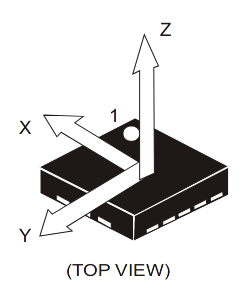
\includegraphics[scale=0.5]{accelaxes}
	\end{center}
\end{figure}
\footnotetext{http://www.st.com/resource/en/datasheet/lis3dsh.pdf}
However, for the purposes of this project, the goal was to transform the raw accelerometer data into
more symbolic quantities. As such, the \textit{pitch} and \textit{roll} measurements were of
interest. These quantities are often associated with the orientation in 3D space of airplanes, for
example. Conventionally, the pitch is defined as the rotation about the $x$ axis, and the roll is
defined as the rotation about the $y$ axis. Thus, letting $a_x, a_y, a_z$ be the acceleration
measurements along the $x$, $y$, and $z$ axes respectively, we may compute pitch as follows:
\begin{equation}
	\mathsf{Pitch}(a_x,a_y,a_z) = \left(\frac{180}{\pi}\right)\arctan\frac{a_x}{\sqrt{a_y^2+a_z^2}}
\end{equation}
where the $180/\pi$ term scales the measurement to degrees from radians. Similarly, we compute the
roll as follows:
\begin{equation}
	\mathsf{Roll}(a_x,a_y,a_z) = \left(\frac{180}{\pi}\right)\arctan\frac{a_y}{\sqrt{a_x^2+a_z^2}}
\end{equation}
\subsection{Communication Between the Two Microcontrollers: UART}
In order to transmit microphone or accelerometer data to eventually reach the web server, it must be
communicated from the Discovery Board to the Nucleo Board, since the Nucleo Board has the ability to
do Bluetooth Low Energy communication. In order to communicate data between the Discovery and the
Nucleo, the Universal Asynchronous Receiver/Transmitter (UART) protocol is used. UART is a very
simple system that allows communication between two devices wired together. Each device requires a
ground pin (\texttt{GND}), a transmission pin (\texttt{TX}), and a receiver pin (\texttt{RX}). Since
the communication is asynchronous, no clock or synchronization lines are required. To distinguish
when a transmission has ceased or begun, special start and end sequences of serial bits are
standardized. Given both the \texttt{RX} and \texttt{TX} lines, however, full duplex communication
is possible. However, for the purposes of this system, full duplex communication was not necessary.
However, bidirectional communication was implemented.\\\\
Using the HAL drivers, communication via UART is very simple. The \texttt{HAL\_UART\_Transmit}
function merely takes a handle to the UART device, a buffer of data, the length of the buffer, and a
timeout period, and transmits the data in the buffer serially on the \texttt{TX} line. Similarly, the
\texttt{HAL\_UART\_Receive} function takes a handle to the UART device, a buffer for data, the
amount $n$ of bytes to receive, and a
timeout period, and fills the buffer with the data read serially from the \texttt{RX} line. This
function call is \textit{blocking}, meaning the program waits for all $n$ bytes to be received before
proceeding. Moreover, the \texttt{HAL\_UART\_Receive\_IT} function was used, which accomplishes the
same task as \texttt{HAL\_UART\_Receive}. However, this function is not blocking, and instead
triggers an interrupt when the $n$ bytes have been received.
\subsection{Bluetooth Low Energy}

Bluetooth low energy (or BLE for short) is a wireless personal area network technology aimed at applications in health care, fitness, security, and home entertainment. 
It allows peripheral devices such as smart phones, medical (heart rate, pressure) sensors and wireless earphones to transmit data within a personal area network. 
Compared to the classic Bluetooth, its purpose is to provide reduced power consumption while maintaining a similar range of communication. 
It saves power by sending small bursts of data as opposed to a continuous stream as used in classic Bluetooth technologies. 
This section of the report details the theory behind BLE and its use cases relevant to the project \cite{gatt}.\\

The purpose of BLE in this project is for it to allow the pair of Nucleo and Discovery boards to communicate data over BLE to a smart phone which then transmits that data to the internet. 
BLE works similarly to Bluetooth, in which a \textit{Central Device} scans for \textit{Peripheral Devices} which \textit{advertise} their personal area networks. 
At this point, once the central and peripheral device connect to one another, one acts as the \textit{Client Device} which receives data from the \textit{Server Device}.\\

For sending data, the server does so by packaging its data within a \textit{Value} under a \textit{Characterstic}, each of which are packaged within a \textit{Service}, this hierarchy of data is part of the \textit{GATT Profile Hierarchy}.\\
One can see this hierarchy within the following \hyperref[fig:uiscreenshot]{Figure \ref{fig:gatt}} \cite{gatt}.\\
\begin{figure}[h]
	\caption{GATT Profile Hierarchy}\label{fig:gatt}
	\begin{center}
		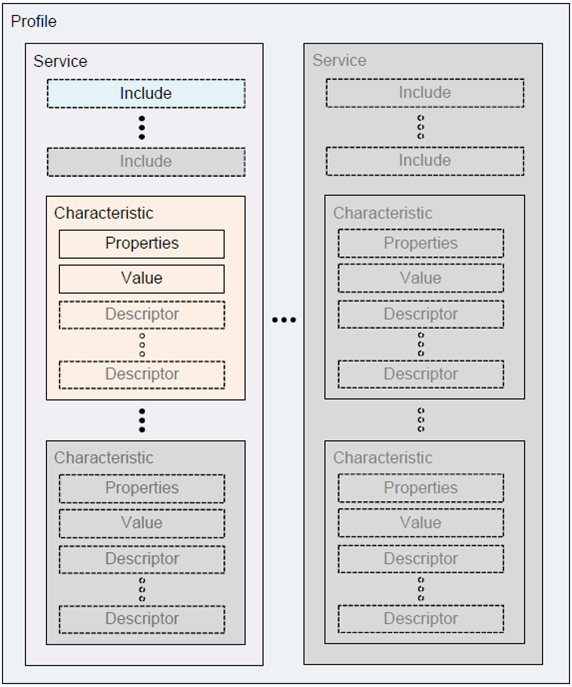
\includegraphics[width=3in]{GATT_Profile_Hierarchy.png}
	\end{center}
\end{figure}

Each server device has only one GATT profile, but within the profile, it may have multiple services, which represent different features. 
For example, one service can be for a heart rate sensor, and another for a pressure sensor. 
In this project, there is only one custom made service. 
A service may have multiple characteristics, which represents different data. 
For example, one characteristic can for a heart rate measurement and one can be for configuration settings for the heart rate sensor.
Within each characteristic, there is a \textit{Value}, the actual data. 
Then there contains one or many \textit{Descriptors}, which describe a value. 
Finally, \textit{Properties} contain the read, write and notify permissions for that characteristic values.\\
